\scanpage{7}

groupe de symétrie $\mathbb Z/2\mathbb Z\times D_5$ d'ordre $20=120/6$

\uline{NB} $6=12/2$

(A)

\textcircled{$A_1$}
\figure{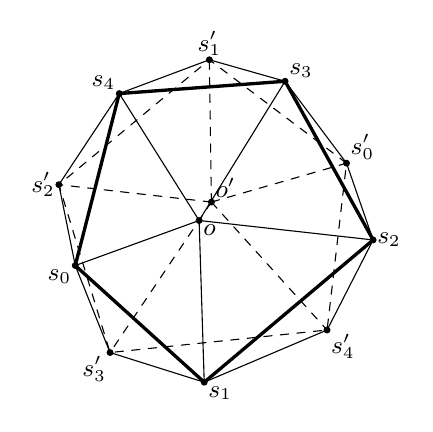
\begin{tikzpicture}[x=0.013cm,y=-0.013cm,line cap=round,line join=round,font=\small]
\coordinate (S0) at (16,201);
\coordinate (S1) at (142,315);
\coordinate (S2) at (307,176);
\coordinate (S3) at (221,21);
\coordinate (S4) at (59,33);
\coordinate (T0) at (281,101);
\coordinate (T1) at (147,0);
\coordinate (T2) at (0,122);
\coordinate (T3) at (50,286);
\coordinate (T4) at (262,264);
\coordinate (O) at (137,157);
\coordinate (Q) at (149,139);
\draw[dashed] (T0)--(T1)--(T2)--(T3)--(T4)--cycle;
\draw[dashed] (Q)--(T0);
\draw[dashed] (Q)--(T1);
\draw[dashed] (Q)--(T2);
\draw[dashed] (Q)--(T3);
\draw[dashed] (Q)--(T4);
\draw (T0)--(S2)--(T4)--(S1)--(T3)--(S0)--(T2)--(S4)--(T1)--(S3)--(T0);
\draw[very thick] (S0)--(S1)--(S2)--(S3)--(S4)--cycle;
\draw (O)--(S0);
\draw (O)--(S1);
\draw (O)--(S2);
\draw (O)--(S3);
\draw (O)--(S4);
\node[below left,inner sep=1.3pt] at (S0) {$s_0$};
\node[below right,inner sep=1.3pt] at (S1) {$s_1$};
\node[right,inner sep=1.3pt] at (S2) {$s_2$};
\node[above right,inner sep=1.3pt] at (S3) {$s_3$};
\node[above left,inner sep=1.3pt] at (S4) {$s_4$};
\node[above right,inner sep=1.3pt] at (T0) {$s'_0$};
\node[above,inner sep=1.3pt] at (T1) {$s'_1$};
\node[left,inner sep=1.3pt] at (T2) {$s'_{2}$};
\node[below left,inner sep=1.3pt] at (T3) {$s'_3$};
\node[below right,inner sep=1.3pt] at (T4) {$s'_4$};
\node[below right,inner sep=1.3pt] at (O) {$o$};
\node[above right,inner sep=1.3pt] at (Q) {$o'$};
\fill (S0) circle[radius=1.25pt];
\fill (S1) circle[radius=1.25pt];
\fill (S2) circle[radius=1.25pt];
\fill (S3) circle[radius=1.25pt];
\fill (S4) circle[radius=1.25pt];
\fill (T0) circle[radius=1.25pt];
\fill (T1) circle[radius=1.25pt];
\fill (T2) circle[radius=1.25pt];
\fill (T3) circle[radius=1.25pt];
\fill (T4) circle[radius=1.25pt];
\fill (Q) circle[radius=1.25pt];
\fill (O) circle[radius=1.25pt];
\end{tikzpicture}}

ou

\figure{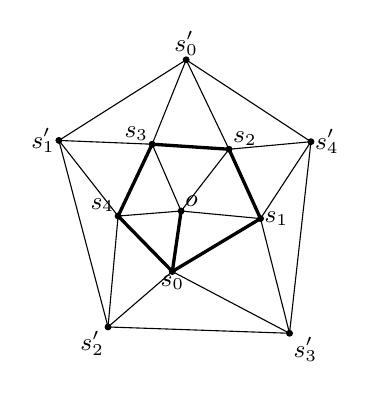
\begin{tikzpicture}[x=0.016cm,y=-0.016cm,line cap=round,line join=round,font=\small]
\coordinate (T0) at (101,0);
\coordinate (T1) at (0,64);
\coordinate (T2) at (39,212);
\coordinate (T3) at (183,217);
\coordinate (T4) at (200,65);
\coordinate (S0) at (90,168);
\coordinate (S1) at (160,126);
\coordinate (S2) at (135,71);
\coordinate (S3) at (74,67);
\coordinate (S4) at (47,124);
\coordinate (O) at (97,120);
\draw (T0)--(T1)--(T2)--(T3)--(T4)--cycle;
\draw (T0)--(S3)--(T1)--(S4)--(T2)--(S0)--(T3)--(S1)--(T4)--(S2)--(T0);
\draw[very thick] (S0)--(S1)--(S2)--(S3)--(S4)--cycle;
\draw[very thick] (O)--(S0);
\draw (O)--(S1);
\draw (O)--(S2);
\draw (O)--(S3);
\draw (O)--(S4);
\node[above,inner sep=1.3pt] at (T0) {$s'_0$};
\node[left,inner sep=1.3pt] at (T1) {$s'_1$};
\node[below left,inner sep=1.3pt] at (T2) {$s'_2$};
\node[below right,inner sep=1.3pt] at (T3) {$s'_3$};
\node[right,inner sep=1.3pt] at (T4) {$s'_4$};
\node[below,inner sep=1.3pt] at (S0) {$s_0$};
\node[right,inner sep=1.3pt] at (S1) {$s_1$};
\node[above right,inner sep=1.3pt] at (S2) {$s_2$};
\node[above left,inner sep=1.3pt] at (S3) {$s_3$};
\node[above left,inner sep=1.3pt] at (S4) {$s_4$};
\node[above right,inner sep=1.3pt] at (O) {$o$};
\fill (T0) circle[radius=1.25pt];
\fill (T1) circle[radius=1.25pt];
\fill (T2) circle[radius=1.25pt];
\fill (T3) circle[radius=1.25pt];
\fill (T4) circle[radius=1.25pt];
\fill (S0) circle[radius=1.25pt];
\fill (S1) circle[radius=1.25pt];
\fill (S2) circle[radius=1.25pt];
\fill (S3) circle[radius=1.25pt];
\fill (S4) circle[radius=1.25pt];
\fill (O) circle[radius=1.25pt];
\end{tikzpicture}}

($\Pi,\Pi'$ deux pent. comb. $\Pi\simeq\Pi'\quad s\longmapsto s'$)

\[
 S=\deleted{\unsure{\{\}}}\inserted{\{o\}\amalg}\Pi\amalg\Pi'\amalg\{o'\}
\]

\diagram{$\begin{array}{llll}
 A=&\left\{\begin{array}{ll}\{o,s\}&s\in\Pi\\\{o',s'\}&s'\in\Pi'\end{array}\right\} &10\\
 &A(\Pi)\quad A(\Pi')&10\\
 &\bigl(\{\underset{\substack{\rotatebox{-90}{$\in$}\\\Pi}}{s},\underset{\substack{\rotatebox{-90}{$\in$}\\\Pi'}}{t}\}\ \unsure{\mid t|\,\not\ni}\,s&10\\
 &\multicolumn{2}{l}{\text{$t$ incident à la face opp. à $s'$}}\\
 &\multicolumn{2}{l}{\text{i.e. }\underset{\substack{\Vert\\\unsure{\delta|d}(t',s)}}{\delta(t,s')}=1}
 \end{array}$}

\textcircled{$A_2$}
\figure{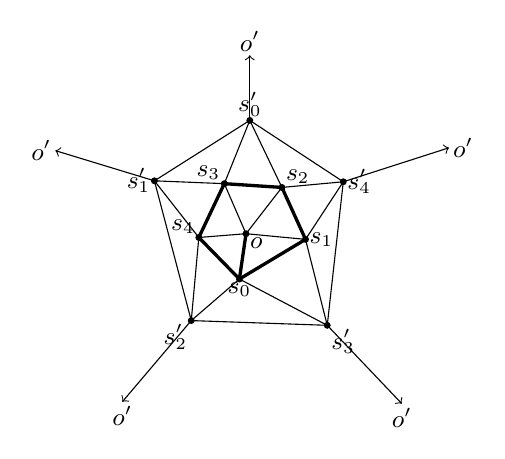
\begin{tikzpicture}[x=0.012cm,y=-0.012cm,line cap=round,line join=round,font=\small]
\coordinate (T0) at (206,69);
\coordinate (T1) at (105,133);
\coordinate (T2) at (144,281);
\coordinate (T3) at (288,286);
\coordinate (T4) at (305,134);
\coordinate (S0) at (195,237);
\coordinate (S1) at (265,195);
\coordinate (S2) at (240,140);
\coordinate (S3) at (179,136);
\coordinate (S4) at (152,193);
\coordinate (O) at (202,189);
\coordinate (E0) at (206,0);
\coordinate (E1) at (0,101);
\coordinate (E2) at (71,367);
\coordinate (E3) at (367,369);
\coordinate (E4) at (417,98);
\draw (T0)--(T1)--(T2)--(T3)--(T4)--cycle;
\draw (T0)--(S3)--(T1)--(S4)--(T2)--(S0)--(T3)--(S1)--(T4)--(S2)--(T0);
\draw[very thick] (S0)--(S1)--(S2)--(S3)--(S4)--cycle;
\draw[very thick] (O)--(S0);
\draw (O)--(S1);
\draw (O)--(S2);
\draw (O)--(S3);
\draw (O)--(S4);
\draw[->] (T0)--(E0);
\draw[->] (T1)--(E1);
\draw[->] (T2)--(E2);
\draw[->] (T3)--(E3);
\draw[->] (T4)--(E4);
\node[above,inner sep=1.3pt] at (T0) {$s'_0$};
\node[left,inner sep=1.3pt] at (T1) {$s'_1$};
\node[below left,inner sep=1.3pt] at (T2) {$s'_2$};
\node[below right,inner sep=1.3pt] at (T3) {$s'_3$};
\node[right,inner sep=1.3pt] at (T4) {$s'_4$};
\node[below,inner sep=1.3pt] at (S0) {$s_0$};
\node[right,inner sep=1.3pt] at (S1) {$s_1$};
\node[above right,inner sep=1.3pt] at (S2) {$s_2$};
\node[above left,inner sep=1.3pt] at (S3) {$s_3$};
\node[above left,inner sep=1.3pt] at (S4) {$s_4$};
\node[below right,inner sep=1.3pt] at (O) {$o$};
\node[above,inner sep=1.3pt] at (E0) {$o'$};
\node[left,inner sep=1.3pt] at (E1) {$o'$};
\node[below,inner sep=1.3pt] at (E2) {$o'$};
\node[below,inner sep=1.3pt] at (E3) {$o'$};
\node[right,inner sep=1.3pt] at (E4) {$o'$};
\fill (T0) circle[radius=1.25pt];
\fill (T1) circle[radius=1.25pt];
\fill (T2) circle[radius=1.25pt];
\fill (T3) circle[radius=1.25pt];
\fill (T4) circle[radius=1.25pt];
\fill (S0) circle[radius=1.25pt];
\fill (S1) circle[radius=1.25pt];
\fill (S2) circle[radius=1.25pt];
\fill (S3) circle[radius=1.25pt];
\fill (S4) circle[radius=1.25pt];
\fill (O) circle[radius=1.25pt];
\end{tikzpicture}}

\noindent\rule{\linewidth}{0.35pt}

\figure{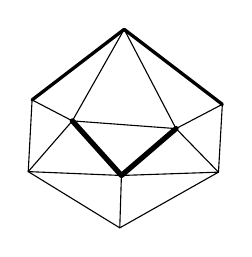
\begin{tikzpicture}[x=0.007cm,y=-0.007cm,line cap=round,line join=round,font=\small]
\coordinate (A) at (174,0);
\coordinate (B) at (0,258);
\coordinate (C) at (345,259);
\coordinate (A1) at (166,360);
\coordinate (B1) at (352,136);
\coordinate (C1) at (7,128);
\coordinate (U) at (169,265);
\coordinate (V) at (268,180);
\coordinate (W) at (80,166);
\coordinate (U1) at (176,121);
\coordinate (V1) at (64,229);
\coordinate (W1) at (282,235);
\draw (A)--(B1)--(C)--(A1)--(B)--(C1)--cycle;
\draw (A)--(W)--(V)--(A);
\draw (B)--(W)--(C1);
\draw (B)--(U)--(C);
\draw (C)--(V)--(B1);
\draw (U)--(A1);
\draw[line width=1.9pt] (W)--(U)--(V);
\draw[very thick] (C1)--(A)--(B1);
\end{tikzpicture}}

\figure{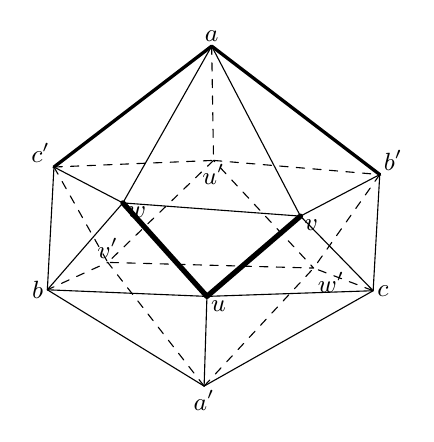
\begin{tikzpicture}[x=0.012cm,y=-0.012cm,line cap=round,line join=round,font=\small]
\coordinate (A) at (174,0);
\coordinate (B) at (0,258);
\coordinate (C) at (345,259);
\coordinate (A1) at (166,360);
\coordinate (B1) at (352,136);
\coordinate (C1) at (7,128);
\coordinate (U) at (169,265);
\coordinate (V) at (268,180);
\coordinate (W) at (80,166);
\coordinate (U1) at (176,121);
\coordinate (V1) at (64,229);
\coordinate (W1) at (282,235);
\draw[dashed] (A)--(U1)--(C1);
\draw[dashed] (U1)--(B1);
\draw[dashed] (U1)--(V1)--(W1)--cycle;
\draw[dashed] (A1)--(V1)--(B);
\draw[dashed] (A1)--(W1)--(C);
\draw[dashed] (C1)--(V1);
\draw[dashed] (B1)--(W1);
\draw (A)--(B1)--(C)--(A1)--(B)--(C1)--cycle;
\draw (A)--(W)--(V)--(A);
\draw (B)--(W)--(C1);
\draw (B)--(U)--(C);
\draw (C)--(V)--(B1);
\draw (U)--(A1);
\draw[line width=1.9pt] (W)--(U)--(V);
\draw[very thick] (C1)--(A)--(B1);
\node[above,inner sep=1.3pt] at (A) {$a$};
\node[left,inner sep=1.3pt] at (B) {$b$};
\node[right,inner sep=1.3pt] at (C) {$c$};
\node[below,inner sep=1.3pt] at (A1) {$a'$};
\node[above right,inner sep=1.3pt] at (B1) {$b'$};
\node[above left,inner sep=1.3pt] at (C1) {$c'$};
\node[below right,inner sep=1.3pt] at (U) {$u$};
\node[below right,inner sep=1.3pt] at (V) {$v$};
\node[below right,inner sep=1.3pt] at (W) {$w$};
\node[below,inner sep=1.3pt] at (U1) {$u'$};
\node[above,inner sep=1.3pt] at (V1) {$v'$};
\node[below right,inner sep=1.3pt] at (W1) {$w'$};
\end{tikzpicture}}

% archive sheet number: 6

